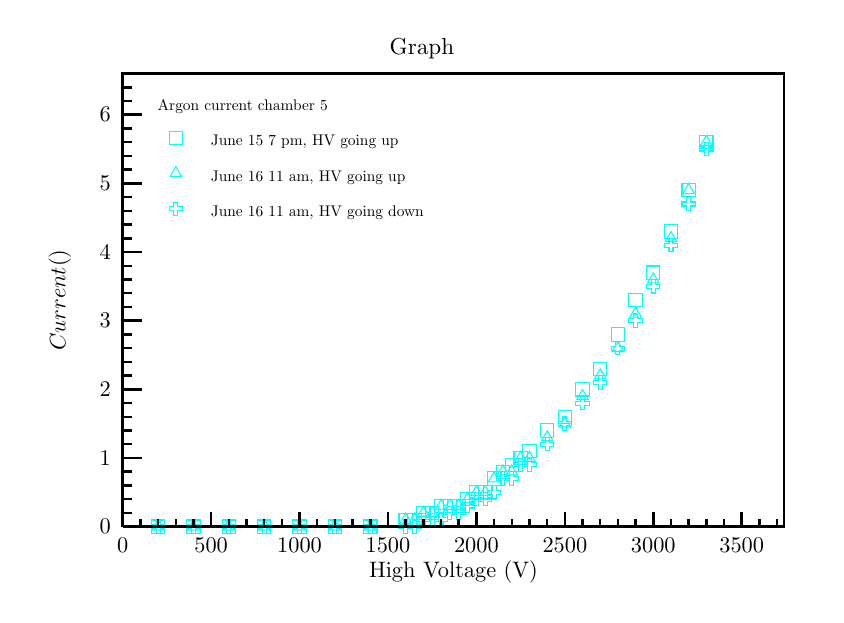
\begin{tikzpicture}
\pgfdeclareplotmark{cross} {
\pgfpathmoveto{\pgfpoint{-0.3\pgfplotmarksize}{\pgfplotmarksize}}
\pgfpathlineto{\pgfpoint{+0.3\pgfplotmarksize}{\pgfplotmarksize}}
\pgfpathlineto{\pgfpoint{+0.3\pgfplotmarksize}{0.3\pgfplotmarksize}}
\pgfpathlineto{\pgfpoint{+1\pgfplotmarksize}{0.3\pgfplotmarksize}}
\pgfpathlineto{\pgfpoint{+1\pgfplotmarksize}{-0.3\pgfplotmarksize}}
\pgfpathlineto{\pgfpoint{+0.3\pgfplotmarksize}{-0.3\pgfplotmarksize}}
\pgfpathlineto{\pgfpoint{+0.3\pgfplotmarksize}{-1.\pgfplotmarksize}}
\pgfpathlineto{\pgfpoint{-0.3\pgfplotmarksize}{-1.\pgfplotmarksize}}
\pgfpathlineto{\pgfpoint{-0.3\pgfplotmarksize}{-0.3\pgfplotmarksize}}
\pgfpathlineto{\pgfpoint{-1.\pgfplotmarksize}{-0.3\pgfplotmarksize}}
\pgfpathlineto{\pgfpoint{-1.\pgfplotmarksize}{0.3\pgfplotmarksize}}
\pgfpathlineto{\pgfpoint{-0.3\pgfplotmarksize}{0.3\pgfplotmarksize}}
\pgfpathclose
\pgfusepathqstroke
}
\pgfdeclareplotmark{cross*} {
\pgfpathmoveto{\pgfpoint{-0.3\pgfplotmarksize}{\pgfplotmarksize}}
\pgfpathlineto{\pgfpoint{+0.3\pgfplotmarksize}{\pgfplotmarksize}}
\pgfpathlineto{\pgfpoint{+0.3\pgfplotmarksize}{0.3\pgfplotmarksize}}
\pgfpathlineto{\pgfpoint{+1\pgfplotmarksize}{0.3\pgfplotmarksize}}
\pgfpathlineto{\pgfpoint{+1\pgfplotmarksize}{-0.3\pgfplotmarksize}}
\pgfpathlineto{\pgfpoint{+0.3\pgfplotmarksize}{-0.3\pgfplotmarksize}}
\pgfpathlineto{\pgfpoint{+0.3\pgfplotmarksize}{-1.\pgfplotmarksize}}
\pgfpathlineto{\pgfpoint{-0.3\pgfplotmarksize}{-1.\pgfplotmarksize}}
\pgfpathlineto{\pgfpoint{-0.3\pgfplotmarksize}{-0.3\pgfplotmarksize}}
\pgfpathlineto{\pgfpoint{-1.\pgfplotmarksize}{-0.3\pgfplotmarksize}}
\pgfpathlineto{\pgfpoint{-1.\pgfplotmarksize}{0.3\pgfplotmarksize}}
\pgfpathlineto{\pgfpoint{-0.3\pgfplotmarksize}{0.3\pgfplotmarksize}}
\pgfpathclose
\pgfusepathqfillstroke
}
\pgfdeclareplotmark{newstar} {
\pgfpathmoveto{\pgfqpoint{0pt}{\pgfplotmarksize}}
\pgfpathlineto{\pgfqpointpolar{44}{0.5\pgfplotmarksize}}
\pgfpathlineto{\pgfqpointpolar{18}{\pgfplotmarksize}}
\pgfpathlineto{\pgfqpointpolar{-20}{0.5\pgfplotmarksize}}
\pgfpathlineto{\pgfqpointpolar{-54}{\pgfplotmarksize}}
\pgfpathlineto{\pgfqpointpolar{-90}{0.5\pgfplotmarksize}}
\pgfpathlineto{\pgfqpointpolar{234}{\pgfplotmarksize}}
\pgfpathlineto{\pgfqpointpolar{198}{0.5\pgfplotmarksize}}
\pgfpathlineto{\pgfqpointpolar{162}{\pgfplotmarksize}}
\pgfpathlineto{\pgfqpointpolar{134}{0.5\pgfplotmarksize}}
\pgfpathclose
\pgfusepathqstroke
}
\pgfdeclareplotmark{newstar*} {
\pgfpathmoveto{\pgfqpoint{0pt}{\pgfplotmarksize}}
\pgfpathlineto{\pgfqpointpolar{44}{0.5\pgfplotmarksize}}
\pgfpathlineto{\pgfqpointpolar{18}{\pgfplotmarksize}}
\pgfpathlineto{\pgfqpointpolar{-20}{0.5\pgfplotmarksize}}
\pgfpathlineto{\pgfqpointpolar{-54}{\pgfplotmarksize}}
\pgfpathlineto{\pgfqpointpolar{-90}{0.5\pgfplotmarksize}}
\pgfpathlineto{\pgfqpointpolar{234}{\pgfplotmarksize}}
\pgfpathlineto{\pgfqpointpolar{198}{0.5\pgfplotmarksize}}
\pgfpathlineto{\pgfqpointpolar{162}{\pgfplotmarksize}}
\pgfpathlineto{\pgfqpointpolar{134}{0.5\pgfplotmarksize}}
\pgfpathclose
\pgfusepathqfillstroke
}
\definecolor{c}{rgb}{1,1,1};
\draw [color=c, fill=c] (0,0) rectangle (10,7.19298);
\definecolor{c}{rgb}{0,0,0};
\draw [c,line width=0.9] (1.2,0.863158) -- (1.2,6.61754) -- (9.6,6.61754) -- (9.6,0.863158) -- (1.2,0.863158);
\draw [c,line width=0.9] (1.2,0.863158) -- (1.2,6.61754) -- (9.6,6.61754) -- (9.6,0.863158) -- (1.2,0.863158);
\draw [c,line width=0.9] (1.2,0.863158) -- (1.2,6.61754) -- (9.6,6.61754) -- (9.6,0.863158) -- (1.2,0.863158);
\draw [c,line width=0.9] (1.2,0.863158) -- (1.2,6.61754) -- (9.6,6.61754) -- (9.6,0.863158) -- (1.2,0.863158);
\draw [c,line width=0.9] (1.2,0.863158) -- (9.6,0.863158);
\draw [c,line width=0.9] (1.2,1.04442) -- (1.2,0.863158);
\draw [c,line width=0.9] (1.4246,0.953789) -- (1.4246,0.863158);
\draw [c,line width=0.9] (1.6492,0.953789) -- (1.6492,0.863158);
\draw [c,line width=0.9] (1.8738,0.953789) -- (1.8738,0.863158);
\draw [c,line width=0.9] (2.0984,0.953789) -- (2.0984,0.863158);
\draw [c,line width=0.9] (2.32299,1.04442) -- (2.32299,0.863158);
\draw [c,line width=0.9] (2.54759,0.953789) -- (2.54759,0.863158);
\draw [c,line width=0.9] (2.77219,0.953789) -- (2.77219,0.863158);
\draw [c,line width=0.9] (2.99679,0.953789) -- (2.99679,0.863158);
\draw [c,line width=0.9] (3.22139,0.953789) -- (3.22139,0.863158);
\draw [c,line width=0.9] (3.44599,1.04442) -- (3.44599,0.863158);
\draw [c,line width=0.9] (3.67059,0.953789) -- (3.67059,0.863158);
\draw [c,line width=0.9] (3.89519,0.953789) -- (3.89519,0.863158);
\draw [c,line width=0.9] (4.11979,0.953789) -- (4.11979,0.863158);
\draw [c,line width=0.9] (4.34439,0.953789) -- (4.34439,0.863158);
\draw [c,line width=0.9] (4.56898,1.04442) -- (4.56898,0.863158);
\draw [c,line width=0.9] (4.79358,0.953789) -- (4.79358,0.863158);
\draw [c,line width=0.9] (5.01818,0.953789) -- (5.01818,0.863158);
\draw [c,line width=0.9] (5.24278,0.953789) -- (5.24278,0.863158);
\draw [c,line width=0.9] (5.46738,0.953789) -- (5.46738,0.863158);
\draw [c,line width=0.9] (5.69198,1.04442) -- (5.69198,0.863158);
\draw [c,line width=0.9] (5.91658,0.953789) -- (5.91658,0.863158);
\draw [c,line width=0.9] (6.14118,0.953789) -- (6.14118,0.863158);
\draw [c,line width=0.9] (6.36578,0.953789) -- (6.36578,0.863158);
\draw [c,line width=0.9] (6.59037,0.953789) -- (6.59037,0.863158);
\draw [c,line width=0.9] (6.81497,1.04442) -- (6.81497,0.863158);
\draw [c,line width=0.9] (7.03957,0.953789) -- (7.03957,0.863158);
\draw [c,line width=0.9] (7.26417,0.953789) -- (7.26417,0.863158);
\draw [c,line width=0.9] (7.48877,0.953789) -- (7.48877,0.863158);
\draw [c,line width=0.9] (7.71337,0.953789) -- (7.71337,0.863158);
\draw [c,line width=0.9] (7.93797,1.04442) -- (7.93797,0.863158);
\draw [c,line width=0.9] (8.16257,0.953789) -- (8.16257,0.863158);
\draw [c,line width=0.9] (8.38717,0.953789) -- (8.38717,0.863158);
\draw [c,line width=0.9] (8.61176,0.953789) -- (8.61176,0.863158);
\draw [c,line width=0.9] (8.83636,0.953789) -- (8.83636,0.863158);
\draw [c,line width=0.9] (9.06096,1.04442) -- (9.06096,0.863158);
\draw [c,line width=0.9] (9.06096,1.04442) -- (9.06096,0.863158);
\draw [c,line width=0.9] (9.28556,0.953789) -- (9.28556,0.863158);
\draw [c,line width=0.9] (9.51016,0.953789) -- (9.51016,0.863158);
\draw [anchor=base] (1.2,0.539474) node[scale=0.807119, color=c, rotate=0]{0};
\draw [anchor=base] (2.32299,0.539474) node[scale=0.807119, color=c, rotate=0]{500};
\draw [anchor=base] (3.44599,0.539474) node[scale=0.807119, color=c, rotate=0]{1000};
\draw [anchor=base] (4.56898,0.539474) node[scale=0.807119, color=c, rotate=0]{1500};
\draw [anchor=base] (5.69198,0.539474) node[scale=0.807119, color=c, rotate=0]{2000};
\draw [anchor=base] (6.81497,0.539474) node[scale=0.807119, color=c, rotate=0]{2500};
\draw [anchor=base] (7.93797,0.539474) node[scale=0.807119, color=c, rotate=0]{3000};
\draw [anchor=base] (9.06096,0.539474) node[scale=0.807119, color=c, rotate=0]{3500};
\draw (5.4,0.287719) node[scale=0.807119, color=c, rotate=0]{High Voltage (V)};
\draw [c,line width=0.9] (1.2,0.863158) -- (1.2,6.61754);
\draw [c,line width=0.9] (1.44,0.863158) -- (1.2,0.863158);
\draw [c,line width=0.9] (1.32,1.03753) -- (1.2,1.03753);
\draw [c,line width=0.9] (1.32,1.21191) -- (1.2,1.21191);
\draw [c,line width=0.9] (1.32,1.38628) -- (1.2,1.38628);
\draw [c,line width=0.9] (1.32,1.56066) -- (1.2,1.56066);
\draw [c,line width=0.9] (1.44,1.73503) -- (1.2,1.73503);
\draw [c,line width=0.9] (1.32,1.90941) -- (1.2,1.90941);
\draw [c,line width=0.9] (1.32,2.08379) -- (1.2,2.08379);
\draw [c,line width=0.9] (1.32,2.25816) -- (1.2,2.25816);
\draw [c,line width=0.9] (1.32,2.43254) -- (1.2,2.43254);
\draw [c,line width=0.9] (1.44,2.60691) -- (1.2,2.60691);
\draw [c,line width=0.9] (1.32,2.78129) -- (1.2,2.78129);
\draw [c,line width=0.9] (1.32,2.95566) -- (1.2,2.95566);
\draw [c,line width=0.9] (1.32,3.13004) -- (1.2,3.13004);
\draw [c,line width=0.9] (1.32,3.30441) -- (1.2,3.30441);
\draw [c,line width=0.9] (1.44,3.47879) -- (1.2,3.47879);
\draw [c,line width=0.9] (1.32,3.65316) -- (1.2,3.65316);
\draw [c,line width=0.9] (1.32,3.82754) -- (1.2,3.82754);
\draw [c,line width=0.9] (1.32,4.00191) -- (1.2,4.00191);
\draw [c,line width=0.9] (1.32,4.17629) -- (1.2,4.17629);
\draw [c,line width=0.9] (1.44,4.35066) -- (1.2,4.35066);
\draw [c,line width=0.9] (1.32,4.52504) -- (1.2,4.52504);
\draw [c,line width=0.9] (1.32,4.69942) -- (1.2,4.69942);
\draw [c,line width=0.9] (1.32,4.87379) -- (1.2,4.87379);
\draw [c,line width=0.9] (1.32,5.04817) -- (1.2,5.04817);
\draw [c,line width=0.9] (1.44,5.22254) -- (1.2,5.22254);
\draw [c,line width=0.9] (1.32,5.39692) -- (1.2,5.39692);
\draw [c,line width=0.9] (1.32,5.57129) -- (1.2,5.57129);
\draw [c,line width=0.9] (1.32,5.74567) -- (1.2,5.74567);
\draw [c,line width=0.9] (1.32,5.92004) -- (1.2,5.92004);
\draw [c,line width=0.9] (1.44,6.09442) -- (1.2,6.09442);
\draw [c,line width=0.9] (1.44,6.09442) -- (1.2,6.09442);
\draw [c,line width=0.9] (1.32,6.26879) -- (1.2,6.26879);
\draw [c,line width=0.9] (1.32,6.44317) -- (1.2,6.44317);
\draw [anchor= east] (1.15,0.863158) node[scale=0.807119, color=c, rotate=0]{0};
\draw [anchor= east] (1.15,1.73503) node[scale=0.807119, color=c, rotate=0]{1};
\draw [anchor= east] (1.15,2.60691) node[scale=0.807119, color=c, rotate=0]{2};
\draw [anchor= east] (1.15,3.47879) node[scale=0.807119, color=c, rotate=0]{3};
\draw [anchor= east] (1.15,4.35066) node[scale=0.807119, color=c, rotate=0]{4};
\draw [anchor= east] (1.15,5.22254) node[scale=0.807119, color=c, rotate=0]{5};
\draw [anchor= east] (1.15,6.09442) node[scale=0.807119, color=c, rotate=0]{6};
\draw (0.4,3.74035) node[scale=0.807119, color=c, rotate=90]{$Current (\muA)$};
\definecolor{c}{rgb}{1,1,1};
\foreach \P in {(1.2,0.863158), (8.83636,6.09442)}{\draw[mark options={color=c,fill=c},mark size=2.402402pt,mark=*,mark size=1pt] plot coordinates {\P};}
\definecolor{c}{rgb}{0,1,1};
\foreach \P in {(1.6492,0.863158), (2.0984,0.863158), (2.54759,0.863158), (2.99679,0.863158), (3.44599,0.863158), (3.89519,0.863158), (4.34439,0.863158), (4.79358,0.950346), (4.90588,0.950346), (5.01818,1.03753), (5.13048,1.03753), (5.24278,1.12472),
 (5.35508,1.12472), (5.46738,1.12472), (5.57968,1.21191), (5.69198,1.2991), (5.80428,1.2991), (5.91658,1.47347), (6.02888,1.56066), (6.14118,1.64785), (6.25348,1.73503), (6.36578,1.82222), (6.59037,2.08379), (6.81497,2.25816), (7.03957,2.60691),
 (7.26417,2.86847), (7.48877,3.30441), (7.71337,3.74035), (7.93797,4.0891), (8.16257,4.61223), (8.38717,5.13535), (8.61176,5.74567)}{\draw[mark options={color=c,fill=c},mark size=2.402402pt,mark=square] plot coordinates {\P};}
\foreach \P in {(1.6492,0.863158), (2.0984,0.863158), (2.54759,0.863158), (2.99679,0.863158), (3.44599,0.863158), (3.89519,0.863158), (4.34439,0.863158), (4.79358,0.950346), (4.90588,0.950346), (5.01818,1.03753), (5.13048,1.03753), (5.24278,1.12472),
 (5.35508,1.12472), (5.46738,1.12472), (5.57968,1.21191), (5.69198,1.2991), (5.80428,1.2991), (5.91658,1.47347), (6.02888,1.56066), (6.14118,1.56066), (6.25348,1.73503), (6.36578,1.73503), (6.59037,1.9966), (6.81497,2.17097), (7.03957,2.51972),
 (7.26417,2.78129), (7.48877,3.13004), (7.71337,3.56598), (7.93797,4.00191), (8.16257,4.52504), (8.38717,5.13535), (8.61176,5.74567)}{\draw[mark options={color=c,fill=c},mark size=2.402402pt,mark=triangle] plot coordinates {\P};}
\foreach \P in {(1.6492,0.863158), (2.0984,0.863158), (2.54759,0.863158), (2.99679,0.863158), (3.44599,0.863158), (3.89519,0.863158), (4.34439,0.863158), (4.79358,0.863158), (4.90588,0.863158), (5.01818,0.950346), (5.13048,0.950346),
 (5.24278,0.950346), (5.35508,1.03753), (5.46738,1.03753), (5.57968,1.12472), (5.69198,1.21191), (5.80428,1.21191), (5.91658,1.2991), (6.02888,1.47347), (6.14118,1.47347), (6.25348,1.64785), (6.36578,1.64785), (6.59037,1.90941), (6.81497,2.17097),
 (7.03957,2.43254), (7.26417,2.6941), (7.48877,3.13004), (7.71337,3.47879), (7.93797,3.91473), (8.16257,4.43785), (8.38717,4.96098), (8.61176,5.65848)}{\draw[mark options={color=c,fill=c},mark size=2.402402pt,mark=cross] plot coordinates {\P};}
\definecolor{c}{rgb}{1,1,1};
\draw [color=c, fill=c] (1.5,4.67544) rectangle (4.5,6.47368);
\definecolor{c}{rgb}{0,0,0};
\draw [anchor=base west] (1.575,6.14775) node[scale=0.556634, color=c, rotate=0]{Argon current chamber 5};
\draw [anchor=base west] (2.25,5.69819) node[scale=0.556634, color=c, rotate=0]{June 15 7 pm, HV going up};
\definecolor{c}{rgb}{0,1,1};
\foreach \P in {(1.875,5.79934)}{\draw[mark options={color=c,fill=c},mark size=2.402402pt,mark=square] plot coordinates {\P};}
\definecolor{c}{rgb}{0,0,0};
\draw [anchor=base west] (2.25,5.24863) node[scale=0.556634, color=c, rotate=0]{June 16 11 am, HV going up};
\definecolor{c}{rgb}{0,1,1};
\foreach \P in {(1.875,5.34978)}{\draw[mark options={color=c,fill=c},mark size=2.402402pt,mark=triangle] plot coordinates {\P};}
\definecolor{c}{rgb}{0,0,0};
\draw [anchor=base west] (2.25,4.79907) node[scale=0.556634, color=c, rotate=0]{June 16 11 am, HV going down};
\definecolor{c}{rgb}{0,1,1};
\foreach \P in {(1.875,4.90022)}{\draw[mark options={color=c,fill=c},mark size=2.402402pt,mark=cross] plot coordinates {\P};}
\definecolor{c}{rgb}{0,0,0};
\draw (5,6.93897) node[scale=0.834951, color=c, rotate=0]{Graph};
\draw [c,line width=0.9] (1.2,0.863158) -- (9.6,0.863158);
\draw [c,line width=0.9] (1.2,1.04442) -- (1.2,0.863158);
\draw [c,line width=0.9] (1.4246,0.953789) -- (1.4246,0.863158);
\draw [c,line width=0.9] (1.6492,0.953789) -- (1.6492,0.863158);
\draw [c,line width=0.9] (1.8738,0.953789) -- (1.8738,0.863158);
\draw [c,line width=0.9] (2.0984,0.953789) -- (2.0984,0.863158);
\draw [c,line width=0.9] (2.32299,1.04442) -- (2.32299,0.863158);
\draw [c,line width=0.9] (2.54759,0.953789) -- (2.54759,0.863158);
\draw [c,line width=0.9] (2.77219,0.953789) -- (2.77219,0.863158);
\draw [c,line width=0.9] (2.99679,0.953789) -- (2.99679,0.863158);
\draw [c,line width=0.9] (3.22139,0.953789) -- (3.22139,0.863158);
\draw [c,line width=0.9] (3.44599,1.04442) -- (3.44599,0.863158);
\draw [c,line width=0.9] (3.67059,0.953789) -- (3.67059,0.863158);
\draw [c,line width=0.9] (3.89519,0.953789) -- (3.89519,0.863158);
\draw [c,line width=0.9] (4.11979,0.953789) -- (4.11979,0.863158);
\draw [c,line width=0.9] (4.34439,0.953789) -- (4.34439,0.863158);
\draw [c,line width=0.9] (4.56898,1.04442) -- (4.56898,0.863158);
\draw [c,line width=0.9] (4.79358,0.953789) -- (4.79358,0.863158);
\draw [c,line width=0.9] (5.01818,0.953789) -- (5.01818,0.863158);
\draw [c,line width=0.9] (5.24278,0.953789) -- (5.24278,0.863158);
\draw [c,line width=0.9] (5.46738,0.953789) -- (5.46738,0.863158);
\draw [c,line width=0.9] (5.69198,1.04442) -- (5.69198,0.863158);
\draw [c,line width=0.9] (5.91658,0.953789) -- (5.91658,0.863158);
\draw [c,line width=0.9] (6.14118,0.953789) -- (6.14118,0.863158);
\draw [c,line width=0.9] (6.36578,0.953789) -- (6.36578,0.863158);
\draw [c,line width=0.9] (6.59037,0.953789) -- (6.59037,0.863158);
\draw [c,line width=0.9] (6.81497,1.04442) -- (6.81497,0.863158);
\draw [c,line width=0.9] (7.03957,0.953789) -- (7.03957,0.863158);
\draw [c,line width=0.9] (7.26417,0.953789) -- (7.26417,0.863158);
\draw [c,line width=0.9] (7.48877,0.953789) -- (7.48877,0.863158);
\draw [c,line width=0.9] (7.71337,0.953789) -- (7.71337,0.863158);
\draw [c,line width=0.9] (7.93797,1.04442) -- (7.93797,0.863158);
\draw [c,line width=0.9] (8.16257,0.953789) -- (8.16257,0.863158);
\draw [c,line width=0.9] (8.38717,0.953789) -- (8.38717,0.863158);
\draw [c,line width=0.9] (8.61176,0.953789) -- (8.61176,0.863158);
\draw [c,line width=0.9] (8.83636,0.953789) -- (8.83636,0.863158);
\draw [c,line width=0.9] (9.06096,1.04442) -- (9.06096,0.863158);
\draw [c,line width=0.9] (9.06096,1.04442) -- (9.06096,0.863158);
\draw [c,line width=0.9] (9.28556,0.953789) -- (9.28556,0.863158);
\draw [c,line width=0.9] (9.51016,0.953789) -- (9.51016,0.863158);
\draw [c,line width=0.9] (1.2,0.863158) -- (1.2,6.61754);
\draw [c,line width=0.9] (1.44,0.863158) -- (1.2,0.863158);
\draw [c,line width=0.9] (1.32,1.03753) -- (1.2,1.03753);
\draw [c,line width=0.9] (1.32,1.21191) -- (1.2,1.21191);
\draw [c,line width=0.9] (1.32,1.38628) -- (1.2,1.38628);
\draw [c,line width=0.9] (1.32,1.56066) -- (1.2,1.56066);
\draw [c,line width=0.9] (1.44,1.73503) -- (1.2,1.73503);
\draw [c,line width=0.9] (1.32,1.90941) -- (1.2,1.90941);
\draw [c,line width=0.9] (1.32,2.08379) -- (1.2,2.08379);
\draw [c,line width=0.9] (1.32,2.25816) -- (1.2,2.25816);
\draw [c,line width=0.9] (1.32,2.43254) -- (1.2,2.43254);
\draw [c,line width=0.9] (1.44,2.60691) -- (1.2,2.60691);
\draw [c,line width=0.9] (1.32,2.78129) -- (1.2,2.78129);
\draw [c,line width=0.9] (1.32,2.95566) -- (1.2,2.95566);
\draw [c,line width=0.9] (1.32,3.13004) -- (1.2,3.13004);
\draw [c,line width=0.9] (1.32,3.30441) -- (1.2,3.30441);
\draw [c,line width=0.9] (1.44,3.47879) -- (1.2,3.47879);
\draw [c,line width=0.9] (1.32,3.65316) -- (1.2,3.65316);
\draw [c,line width=0.9] (1.32,3.82754) -- (1.2,3.82754);
\draw [c,line width=0.9] (1.32,4.00191) -- (1.2,4.00191);
\draw [c,line width=0.9] (1.32,4.17629) -- (1.2,4.17629);
\draw [c,line width=0.9] (1.44,4.35066) -- (1.2,4.35066);
\draw [c,line width=0.9] (1.32,4.52504) -- (1.2,4.52504);
\draw [c,line width=0.9] (1.32,4.69942) -- (1.2,4.69942);
\draw [c,line width=0.9] (1.32,4.87379) -- (1.2,4.87379);
\draw [c,line width=0.9] (1.32,5.04817) -- (1.2,5.04817);
\draw [c,line width=0.9] (1.44,5.22254) -- (1.2,5.22254);
\draw [c,line width=0.9] (1.32,5.39692) -- (1.2,5.39692);
\draw [c,line width=0.9] (1.32,5.57129) -- (1.2,5.57129);
\draw [c,line width=0.9] (1.32,5.74567) -- (1.2,5.74567);
\draw [c,line width=0.9] (1.32,5.92004) -- (1.2,5.92004);
\draw [c,line width=0.9] (1.44,6.09442) -- (1.2,6.09442);
\draw [c,line width=0.9] (1.44,6.09442) -- (1.2,6.09442);
\draw [c,line width=0.9] (1.32,6.26879) -- (1.2,6.26879);
\draw [c,line width=0.9] (1.32,6.44317) -- (1.2,6.44317);
\draw [c,line width=0.9] (1.2,0.863158) -- (1.2,6.61754) -- (9.6,6.61754) -- (9.6,0.863158) -- (1.2,0.863158);
\draw [c,line width=0.9] (1.2,0.863158) -- (1.2,6.61754) -- (9.6,6.61754) -- (9.6,0.863158) -- (1.2,0.863158);
\end{tikzpicture}
